 \subsection{Obrázky}

    %ukázka zápisu kódu pro obrázek
    %parametr H říká že to bude přímo na tom místě kde je v textu...více http://en.wikibooks.org/wiki/LaTeX/Floats,_Figures_and_Captions
    \begin{figure}[H]
      \centering
      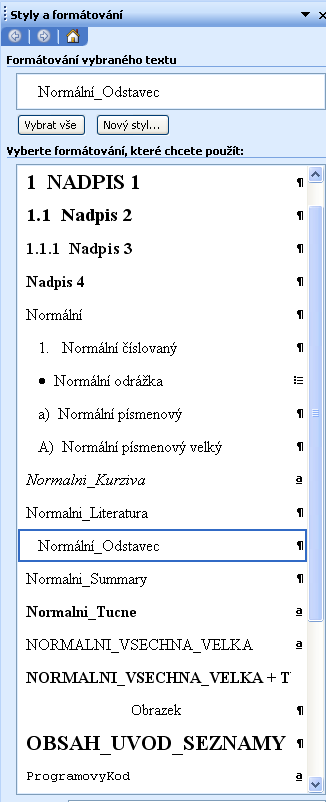
\includegraphics[width=0.2\textwidth]{./obrazky/obrazek_1.png}
      \caption {Styly (převzato z: \cite{Celikyilmaz2009})}
      \label{fig:44}
    \end{figure}

    %ukázka odkazu na zkratky a obrázek
    \Gls{GIT} \Gls{CAD} bla bla bla \odkazObrazek{fig:44}. Pokud chceme uvést překlad z angličtiny můžeme to udělat takto \transl{english words}.

    %dají se dělat i složené obrázky
    \begin{figure}
        \centering
        \begin{subfigure}[b]{0.45\textwidth}
          \centering
          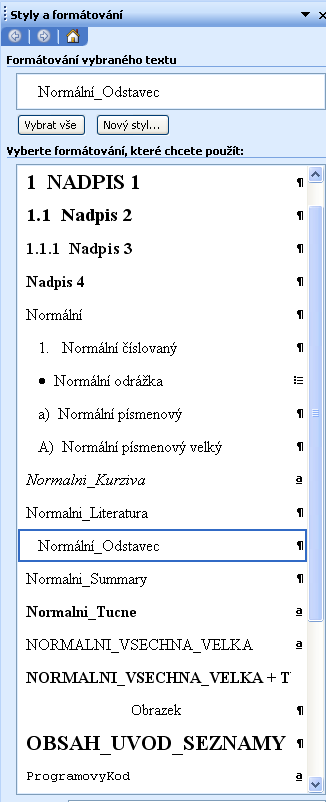
\includegraphics[width=\textwidth]{./obrazky/obrazek_1.png}
          \caption{Cena za metr čtvereční bytů v Londýně (převzato z:\cite{Fotheringham2002})}
          \label{fig2.1}
        \end{subfigure}%
        \quad %add desired spacing between images, e. g. ~, \quad, \qquad etc.
          %(or a blank line to force the subfigure onto a new line)
        \begin{subfigure}[b]{0.45\textwidth}
          \centering
          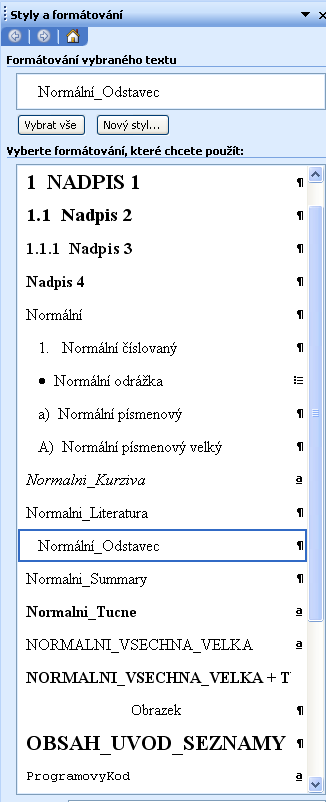
\includegraphics[width=\textwidth]{./obrazky/obrazek_1.png}
          \caption{Obsah zinku v půdě (převzato z:\cite{Hengl2009})}
          \label{fig2.2}
        \end{subfigure}
        \caption{Povrch socioekonomického (a) a fyzickogeografického (b) ukazatele}
        \label{fig2}
    \end{figure}

    \begin{table}[h]
    \caption {Ukázková tabulka}
    \label{tab1}
    \centering
      \begin{tabular}{ |l|l|l| }
        \hline
        \multicolumn{3}{ |c| }{Team sheet} \\
        \hline
        Goalkeeper & GK & Paul Robinson \\ \hline
        \multirow{4}{*}{Defenders} & LB & Lucus Radebe \\
        & DC & Michael Duberry \\
        & DC & Dominic Matteo \\
        & RB & Didier Domi \\ \hline
        \multirow{3}{*}{Midfielders} & MC & David Batty \\
        & MC & Eirik Bakke \\
        & MC & Jody Morris \\ \hline
        Forward & FW & Jamie McMaster \\ \hline
        \multirow{2}{*}{Strikers} & ST & Alan Smith \\
        & ST & Mark Viduka \\
        \hline
      \end{tabular}
    \end{table}

    Odkaz na tabulku pak vytvoříme takto: \odkazTabulka{tab1}.

    \begin{equation}
    \label{eq1}
    c = \sqrt{a^2 + b^2}
    \end{equation}

    Vzorce pak odkazujeme \odkazVzorec{eq1}. 

    Citace se dají dělat buď jako \citep{Talasova2003} nebo \cite{Talasova2003}.


